\section{马尔可夫决策过程}

\figref{fig:rl_pic} 介绍了强化学习中智能体与环境之间的交互过程,智能体观测到环境的状态后,它会采取动作,然后环境根据智能体采取的动作进入到下一个状态,并反馈出对应的奖励信号。举一个踢足球的例子,假设我们一开始什么也不会,但想要学习罚点球,也就是在点球点处将球踢进球门里去,每次练习开始我们观测到球和球门的位置,并尝试调整角度将球踢出去。踢出去之后球的位置会发生变化,根据球和球门的位置我们可以接收到反馈,比如球是进球门了还是踢飞了。接着我们将球重新放回点球点处继续练习,并根据上一次收到的反馈调整我们的射门动作,如此循环交互,直到学会将球踢进球门为止。在这个过程中,我们人就相当于是智能体,球和球门的位置就是人观测到的状态,将球踢出去就是一个动作,而球、球门和球场组成整个环境,每次采取动作后接收到的反馈可以数值化成一个奖励信号,进球门了就是正的奖励,踢飞了或者没踢进就是负的奖励,也就是惩罚。生活中的很多问题都可以用这样一段持续的交互过程来描述,而这个交互过程在数学上可以用马尔可夫决策过程(Markov decision process,MDP),而用于解决 MDP 问题的方法都可以被认为是强化学习方法,因此\kw{ MDP 是强化学习的基本问题模型之一}。换句话说,要想用强化学习算法解决某个实际问题,我们必须首先将这个问题描述或者建模成一个马尔可夫决策过程。顺便说一句,之所以说MDP 是强化学习的基本问题模型之一,这里之一的意思是在更多复杂的情况中比如多智能体环境我们需要把问题建模成一个 MDP 的衍生版本,比如 部分可观测马尔可夫决策过程(partially observable Markov decision processes,POMDP) 以及马尔可夫博弈等等,但广义上来说都属于马尔可夫决策过程,具体在后面讲述相关内容时再详细展开。


\begin{figure}[hbt]
  \centering
  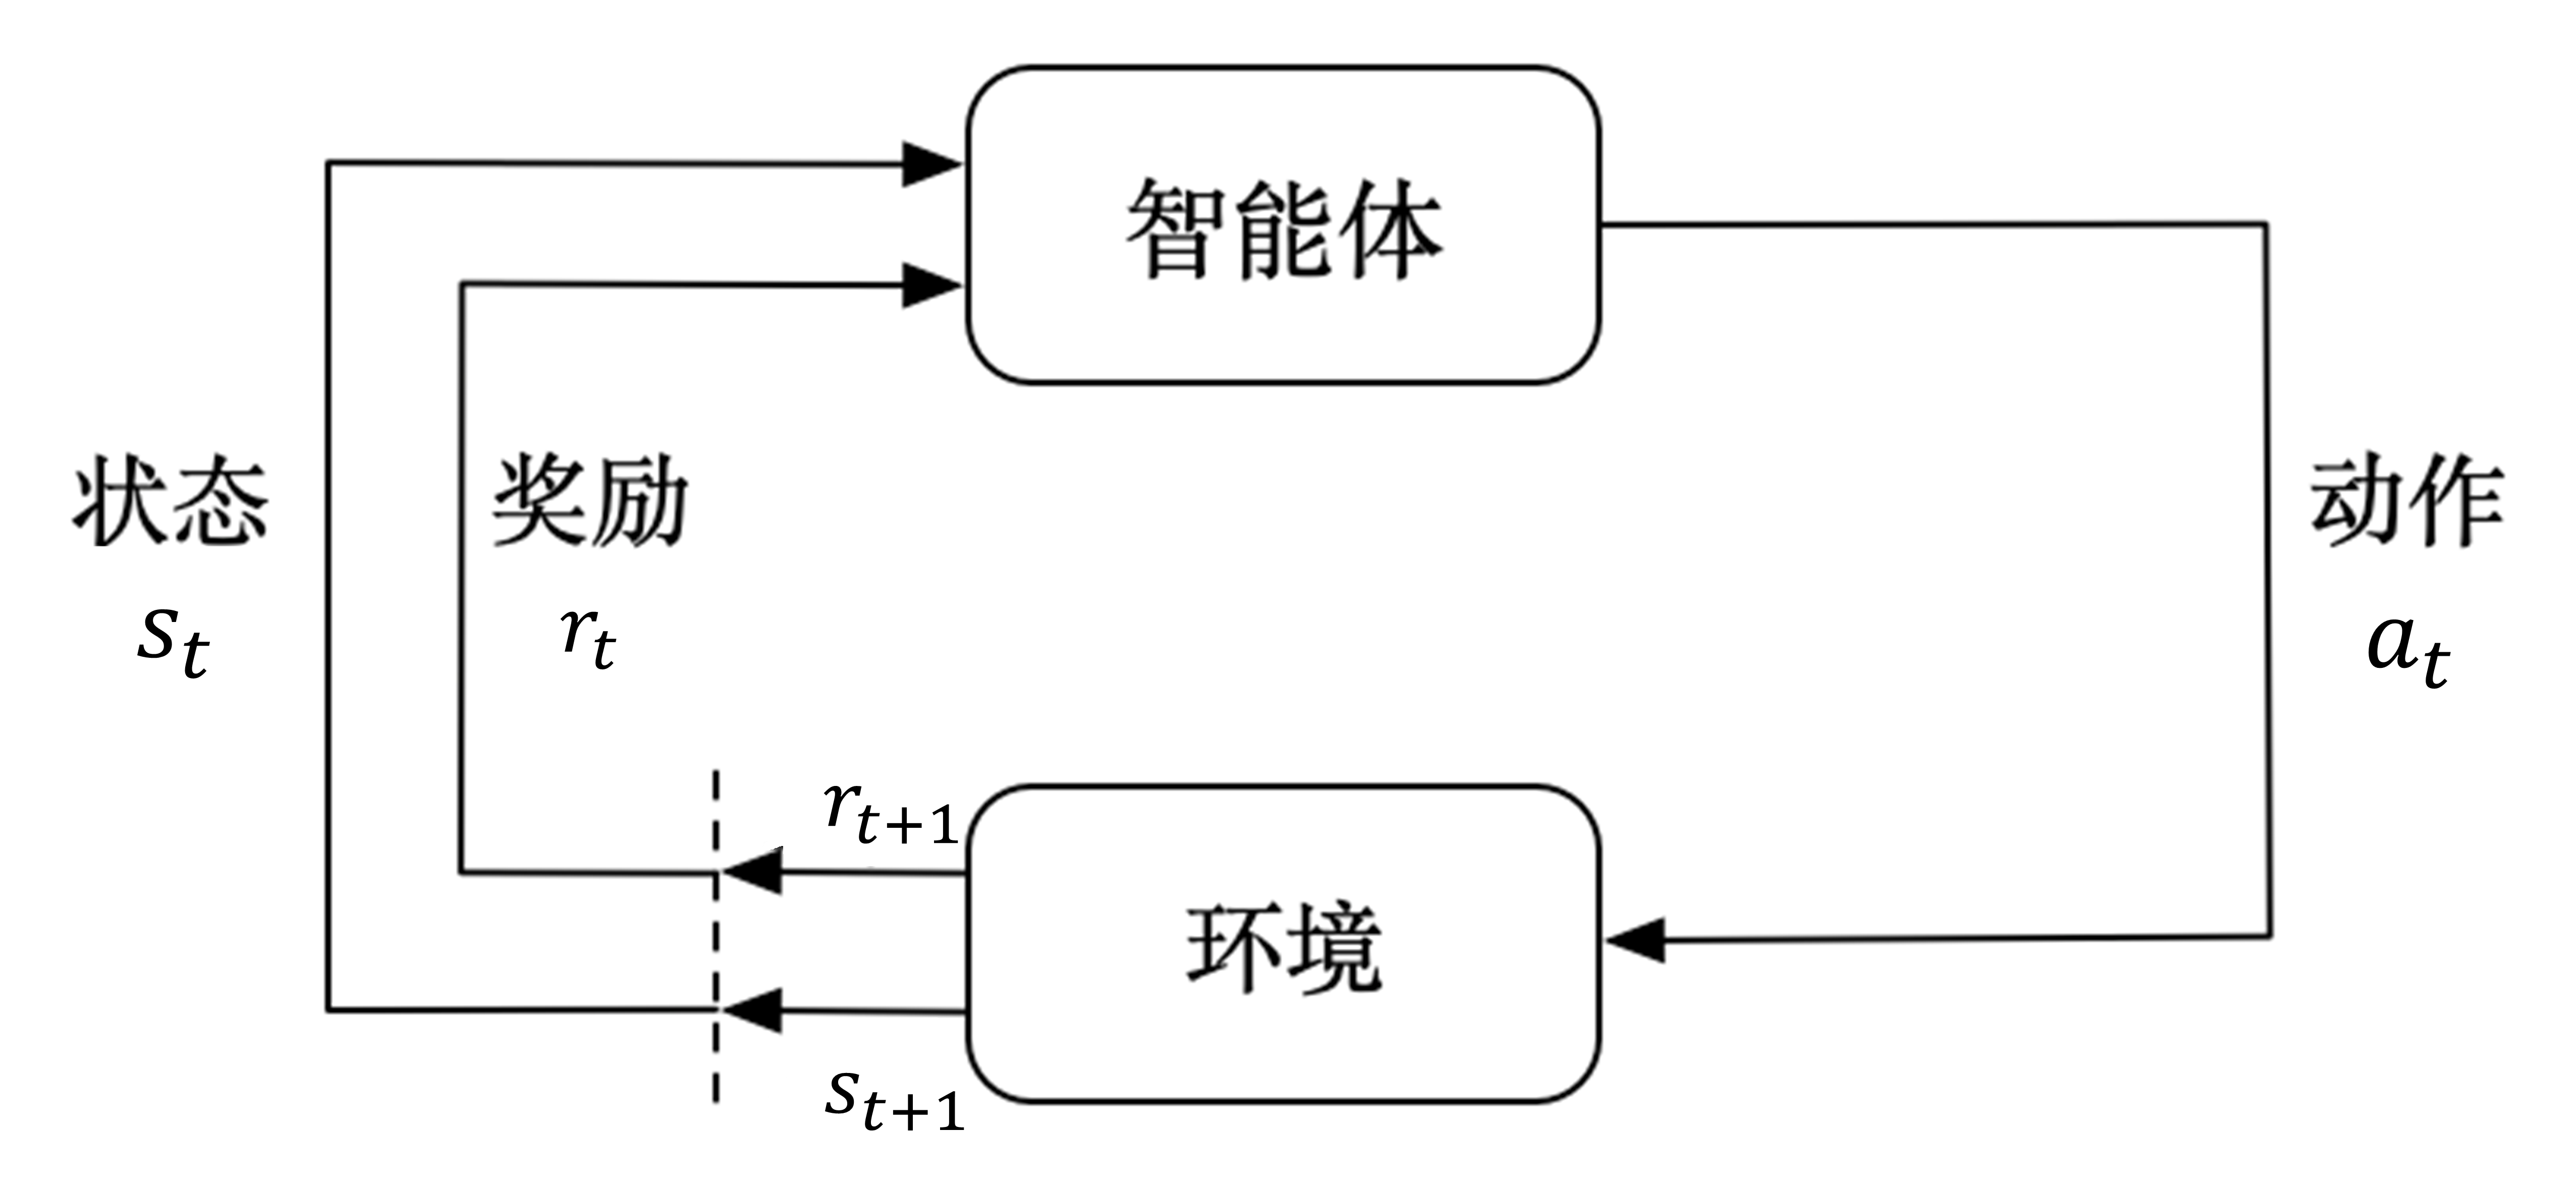
\includegraphics[width=0.5\linewidth]{ch2/figs/rl_pic.png}
  \caption{智能体与环境之间的交互}
  \label{fig:rl_pic}
\end{figure}


本章将介绍马尔可夫决策过程(Markov decision process,MDP)。在介绍马尔可夫决策过程之前,我们先介绍它的简化版本:马尔可夫过程(Markov process,MP)以及马尔可夫奖励过程(Markov reward process,MRP)。通过这两种过程的铺垫,我们可以更容易理解马尔可夫决策过程。
\subsection{马尔可夫过程}
\subsubsection{马尔可夫性质}
\kw{马尔可夫性质(Markov property)}是概率论中的一个概念,指的是当一个随机过程在给定当前状态及所有过去状态情况下,其未来状态的条件概率分布仅依赖于当前状态。换句话说,在给定当前状态下,它与过去状态(即该过程的历史路径)是条件独立的。

以离散随机过程为例,假设随机变量 $X_0,X_1,\cdots,X_T$构成一个随机过程。这些随机变量的所有可能取值的集合被称为状态空间(state space)。如果 $X_{t+1}$ 对于过去状态的条件概率分布仅是 $X_t$ 的一个函数,则
\begin{equation}
  \label{eq:}
  p\left(X_{t+1}=x_{t+1} \mid X_{0:t}=x_{0: t}\right)=p\left(X_{t+1}=x_{t+1} \mid X_{t}=x_{t}\right)
\end{equation}
其中,$X_{0:t}$ 表示变量集合 $X_{0}, X_{1}, \cdots, X_{t}$,$x_{0: t}$ 为在状态空间中的状态序列 $x_{0}, x_{1}, \cdots, x_{t}$。

马尔可夫性质是所有马尔可夫过程的基础。这种性质看似深奥,其实在我们日常生活中也司空见惯,比如一天内,我晚餐的食量由午餐的时间和摄入直接决定,而不由早餐的时间和摄入间接决定(因为早餐摄入的食物在晚餐前就已经消化掉了),这样一来一日三餐的摄入就可以简单看作一个马尔可夫过程。

\subsubsection{马尔可夫链}
% 如果一个状态转移是符合马尔可夫的,也就是满足条件:
马尔可夫过程是一组具有马尔可夫性质的随机变量序列 $s_1,\cdots,s_t$,其中下一个时刻的状态$s_{t+1}$只取决于当前状态 $s_t$。我们设状态的历史为 $h_{t}=\left\{s_{1}, s_{2}, s_{3}, \ldots, s_{t}\right\}$($h_t$ 包含了之前的所有状态),则马尔可夫过程满足条件:
\begin{equation}
  \label{eq:}
  p\left(s_{t+1} \mid s_{t}\right) =p\left(s_{t+1} \mid h_{t}\right)
\end{equation}
从当前 $s_t$ 转移到 $s_{t+1}$,它是直接就等于它之前所有的状态转移到 $s_{t+1}$。

离散时间的马尔可夫过程也称为\kw{马尔可夫链(Markov chain)}。马尔可夫链是最简单的马尔可夫过程,其状态是有限的。例如,\figref{fig:mp_example} 里面有4个状态,这4个状态在 $s_1,s_2,s_3,s_4$ 之间互相转移。比如从 $s_1$ 开始,$s_1$ 有 0.1 的概率继续存留在 $s_1$ 状态,有 0.2 的概率转移到 $s_2$,有 0.7 的概率转移到 $s_4$ 。如果 $s_4$ 是我们的当前状态,它有 0.3 的概率转移到 $s_2$,有 0.2 的概率转移到 $s_3$,有 0.5 的概率留在当前状态。

\begin{figure}[htb]
  \centering
  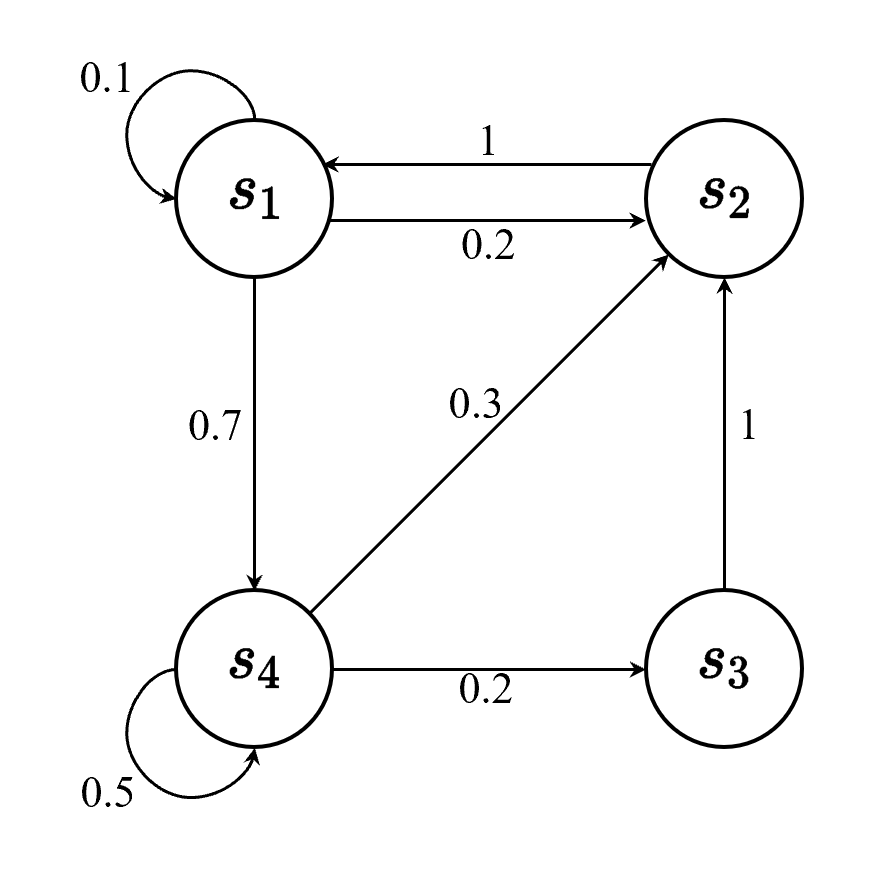
\includegraphics[width=0.3\linewidth]{ch2/figs/m_chain_example.png}
  \caption{马尔可夫链示例}
  \label{fig:mp_example}
\end{figure}

我们可以用\kw{状态转移矩阵(state transition matrix)}$\boldsymbol{P}$ 来描述状态转移 $p\left(s_{t+1}=s^{\prime} \mid s_{t}=s\right)$:
\begin{equation}
  \boldsymbol{P}=\left(\begin{array}{cccc}
    p\left(s_{1} \mid s_{1}\right) & p\left(s_{2} \mid s_{1}\right) & \ldots & p\left(s_{N} \mid s_{1}\right) \\
    p\left(s_{1} \mid s_{2}\right) & p\left(s_{2} \mid s_{2}\right) & \ldots & p\left(s_{N} \mid s_{2}\right) \\
    \vdots & \vdots & \ddots & \vdots \\
    p\left(s_{1} \mid s_{N}\right) & p\left(s_{2} \mid s_{N}\right) & \ldots & p\left(s_{N} \mid s_{N}\right)
    \end{array}\right)
  \label{eq:1}
\end{equation}
状态转移矩阵类似于条件概率(conditional probability),它表示当我们知道当前我们在状态 $s_t$ 时,到达下面所有状态的概率。所以它的每一行描述的是从一个节点到达所有其他节点的概率。

\subsection{马尔可夫奖励过程} 

\kw{马尔可夫奖励过程(Markov reward process, MRP)}是马尔可夫链加上奖励函数。在马尔可夫奖励过程中,状态转移矩阵和状态都与马尔可夫链一样,只是多了\kw{奖励函数(reward function)}。奖励函数 $R$ 是一个期望,表示当我们到达某一个状态的时候,可以获得多大的奖励。这里另外定义了折扣因子 $\gamma$ 。如果状态数是有限的,那么 $R$ 可以是一个向量。

\subsubsection{回报与价值函数}

这里我们进一步定义一些概念。\kw{范围(horizon)} 是指一个回合的长度(每个回合最大的时间步数),它是由有限个步数决定的。
\kw{回报(return)}可以定义为奖励的逐步叠加,假设时刻$t$后的奖励序列为$r_{t+1},r_{t+2},r_{t+3},\cdots$,则回报为
\begin{equation}
  G_{t}=r_{t+1}+\gamma r_{t+2}+\gamma^{2} r_{t+3}+\gamma^{3} r_{t+4}+\ldots+\gamma^{T-t-1} r_{T}
  \label{eq:}
\end{equation}
其中,$T$是最终时刻,$\gamma$ 是折扣因子,越往后得到的奖励,折扣越多。这说明我们更希望得到现有的奖励,对未来的奖励要打折扣。
当我们有了回报之后,就可以定义状态的价值了,就是\kw{状态价值函数(state-value function)}。对于马尔可夫奖励过程,状态价值函数被定义成回报的期望,即
\begin{equation}
  \begin{aligned}
    V^{t}(s) &=\mathbb{E}\left[G_{t} \mid s_{t}=s\right] \\
    &=\mathbb{E}\left[r_{t+1}+\gamma r_{t+2}+\gamma^{2} r_{t+3}+\ldots+\gamma^{T-t-1} r_{T} \mid s_{t}=s\right]
    \end{aligned}
  \label{eq:}
\end{equation}
其中,$G_t$ 是之前定义的\kw{折扣回报(discounted return)}。我们对$G_t$取了一个期望,期望就是从这个状态开始,我们可能获得多大的价值。所以期望也可以看成未来可能获得奖励的当前价值的表现,就是当我们进入某一个状态后,我们现在有多大的价值。

我们使用折扣因子的原因如下。第一,有些马尔可夫过程是带环的,它并不会终结,我们想避免无穷的奖励。第二,我们并不能建立完美的模拟环境的模型,我们对未来的评估不一定是准确的,我们不一定完全信任模型,因为这种不确定性,所以我们对未来的评估增加一个折扣。我们想把这个不确定性表示出来,希望尽可能快地得到奖励,而不是在未来某一个点得到奖励。
第三,如果奖励是有实际价值的,我们可能更希望立刻就得到奖励,而不是后面再得到奖励(现在的钱比以后的钱更有价值)。
最后,我们也更想得到即时奖励。有些时候可以把折扣因子设为 0($\gamma=0$),我们就只关注当前的奖励。
我们也可以把折扣因子设为 1($\gamma=1$),对未来的奖励并没有打折扣,未来获得的奖励与当前获得的奖励是一样的。
折扣因子可以作为强化学习智能体的一个超参数(hyperparameter)来进行调整,通过调整折扣因子,我们可以得到不同动作的智能体。

在马尔可夫奖励过程里面,我们如何计算价值呢?如\figref{fig:fig2.11} 所示,马尔可夫奖励过程依旧是状态转移,其奖励函数可以定义为:智能体进入第一个状态 $s_1$ 的时候会得到 5 的奖励,进入第七个状态 $s_7$ 的时候会得到 10 的奖励,进入其他状态都没有奖励。我们可以用向量来表示奖励函数,即

\begin{equation}
  \label{eq:}
  \boldsymbol{R}=[5,0,0,0,0,0,10]
\end{equation}

\begin{figure}[hbt]
  \centering
  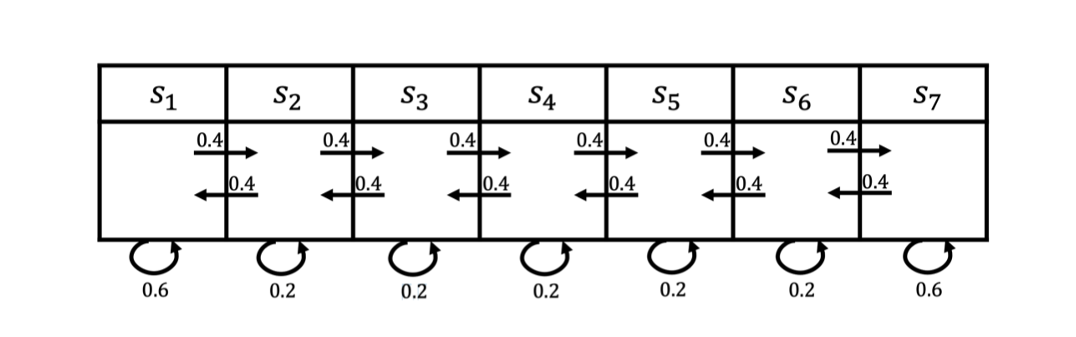
\includegraphics[width=0.7\linewidth]{ch2/figs/2.11.png}
  \caption{马尔可夫奖励过程的例子}
  \label{fig:fig2.11}
\end{figure}

我们对 4 步的回合($\gamma=0.5$)来采样回报 $G$。
% \begin{enumerate}[label=\protect\circled{\arabic*}]

  (1)$s_{4}, s_{5}, s_{6}, s_{7} \text{的回报}: 0+0.5\times 0+0.25 \times 0+ 0.125\times 10=1.25$

  (2)$s_{4}, s_{3}, s_{2}, s_{1} \text{的回报}: 0+0.5 \times 0+0.25\times 0+0.125 \times 5=0.625$

  (3)$s_{4}, s_{5}, s_{6}, s_{6} \text{的回报}: 0+0.5\times 0 +0.25 \times 0+0.125 \times 0=0$
% \end{enumerate}

我们现在可以计算每一个轨迹得到的奖励,比如我们对轨迹 $s_4,s_5,s_6,s_7$ 的奖励进行计算,这里折扣因子是 0.5。
在 $s_4$ 的时候,奖励为0。
下一个状态 $s_5$ 的时候,因为我们已经到了下一步,所以要把 $s_5$ 进行折扣,$s_5$ 的奖励也是0。
然后是 $s_6$,奖励也是0,折扣因子应该是0.25。
到达 $s_7$ 后,我们获得了一个奖励,但是因为状态 $s_7$ 的奖励是未来才获得的奖励,所以我们要对之进行3次折扣。
最终这个轨迹的回报就是 1.25。类似地,我们可以得到其他轨迹的回报。

这里就引出了一个问题,当我们有了一些轨迹的实际回报时,怎么计算它的价值函数呢?比如我们想知道 $s_4$ 的价值,即当我们进入 $s_4$ 后,它的价值到底如何?一个可行的做法就是我们可以生成很多轨迹,然后把轨迹都叠加起来。比如我们可以从 $s_4$ 开始,采样生成很多轨迹,把这些轨迹的回报都计算出来,然后将其取平均值作为我们进入 $s_4$ 的价值。这其实是一种计算价值函数的办法,也就是通过蒙特卡洛(Monte Carlo,MC)采样的方法计算 $s_4$ 的价值。

\subsubsection{马尔可夫奖励过程的例子} 

如\figref{fig:mrp_example} 所示,如果我们在马尔可夫链上加上奖励,那么到达每个状态,我们都会获得一个奖励。我们可以设置对应的奖励,比如智能体到达状态 $s_1$时,可以获得 5 的奖励;到达 $s_7$ 的时候,可以得到 10 的奖励;到达其他状态没有任何奖励。
因为这里的状态是有限的,所以我们可以用向量 $\boldsymbol{R}=[5,0,0,0,0,0,10]$ 来表示奖励函数,$\boldsymbol{R}$表示每个状态的奖励大小。

我们通过一个形象的例子来理解马尔可夫奖励过程。我们把一艘纸船放到河流之中,它就会随着水流而流动,它自身是没有动力的。所以我们可以把马尔可夫奖励过程看成一个随波逐流的例子,当我们从某一个点开始的时候,纸船就会随着事先定义好的状态转移进行流动,它到达每个状态后,我们都有可能获得一些奖励。

\begin{figure}[hbt]
  \centering
  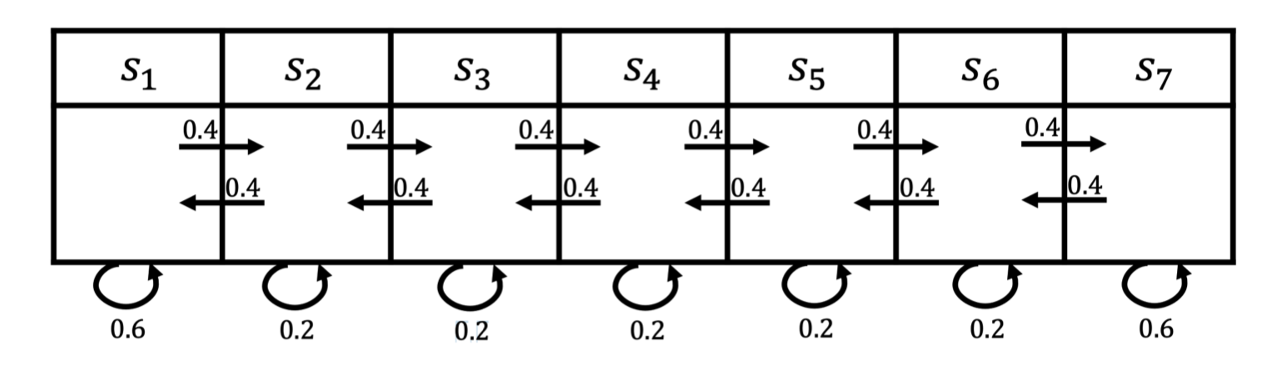
\includegraphics[width=0.5\linewidth]{ch2/figs/2.8}
  \caption{马尔可夫奖励过程的例子}
  \label{fig:mrp_example}
\end{figure}

\subsection{马尔可夫决策过程} 
相对于马尔可夫奖励过程,马尔可夫决策过程多了决策(决策是指动作),其他的定义与马尔可夫奖励过程的是类似的。此外,状态转移也多了一个条件,变成了$p\left(s_{t+1}=s^{\prime} \mid s_{t}=s,a_{t}=a\right)$。未来的状态不仅依赖于当前的状态,也依赖于在当前状态智能体采取的动作。马尔可夫决策过程满足条件:
\begin{equation}
  \label{eq:}
  p\left(s_{t+1} \mid s_{t}, a_{t}\right) =p\left(s_{t+1} \mid h_{t}, a_{t}\right)   
\end{equation}

对于奖励函数,它也多了一个当前的动作,变成了 $R\left(s_{t}=s, a_{t}=a\right)=\mathbb{E}\left[r_{t} \mid s_{t}=s, a_{t}=a\right]$。当前的状态以及采取的动作会决定智能体在当前可能得到的奖励多少。


\subsubsection{马尔可夫决策过程中的策略} 

策略定义了在某一个状态应该采取什么样的动作。知道当前状态后,我们可以把当前状态代入策略函数来得到一个概率,即 
\begin{equation}
  \pi(a \mid s)=p\left(a_{t}=a \mid s_{t}=s\right)
  \label{eq:}
\end{equation}
概率代表在所有可能的动作里面怎样采取行动,比如可能有 0.7 的概率往左走,有 0.3 的概率往右走,这是一个概率的表示。
另外策略也可能是确定的,它有可能直接输出一个值,或者直接告诉我们当前应该采取什么样的动作,而不是一个动作的概率。
假设概率函数是平稳的(stationary),不同时间点,我们采取的动作其实都是在对策略函数进行采样。

已知马尔可夫决策过程和策略 $\pi$,我们可以把马尔可夫决策过程转换成马尔可夫奖励过程。
在马尔可夫决策过程里面,状态转移函数 $P(s'|s,a)$ 基于它当前的状态以及它当前的动作。因为我们现在已知策略函数,也就是已知在每一个状态下,可能采取的动作的概率,所以我们就可以直接把动作进行加和,去掉 $a$,这样我们就可以得到对于马尔可夫奖励过程的转移,这里就没有动作,即
\begin{equation}
  P_{\pi}\left(s^{\prime} \mid s\right)=\sum_{a \in A} \pi(a \mid s) p\left(s^{\prime} \mid s, a\right)
  \label{eq:}
\end{equation}

对于奖励函数,我们也可以把动作去掉,这样就会得到类似于马尔可夫奖励过程的奖励函数,即
\begin{equation}
  r_{\pi}(s)=\sum_{a \in A} \pi(a \mid s) R(s, a)
  \label{eq:}
\end{equation}

\subsubsection{马尔可夫决策过程和马尔可夫过程/马尔可夫奖励过程的区别} 
马尔可夫决策过程里面的状态转移与马尔可夫奖励过程以及马尔可夫过程的状态转移的差异如\figref{fig:fig2.21} 所示。
马尔可夫过程/马尔可夫奖励过程的状态转移是直接决定的。比如当前状态是 $s$,那么直接通过转移概率决定下一个状态是什么。
但对于马尔可夫决策过程,它的中间多了一层动作 $a$ ,即智能体在当前状态的时候,首先要决定采取某一种动作,这样我们会到达某一个黑色的节点。到达这个黑色的节点后,因为有一定的不确定性,所以当智能体当前状态以及智能体当前采取的动作决定过后,智能体进入未来的状态其实也是一个概率分布。在当前状态与未来状态转移过程中多了一层决策性,这是马尔可夫决策过程与之前的马尔可夫过程/马尔可夫奖励过程很不同的一点。在马尔可夫决策过程中,动作是由智能体决定的,智能体会采取动作来决定未来的状态转移。

\begin{figure}[hbt]
  \centering
  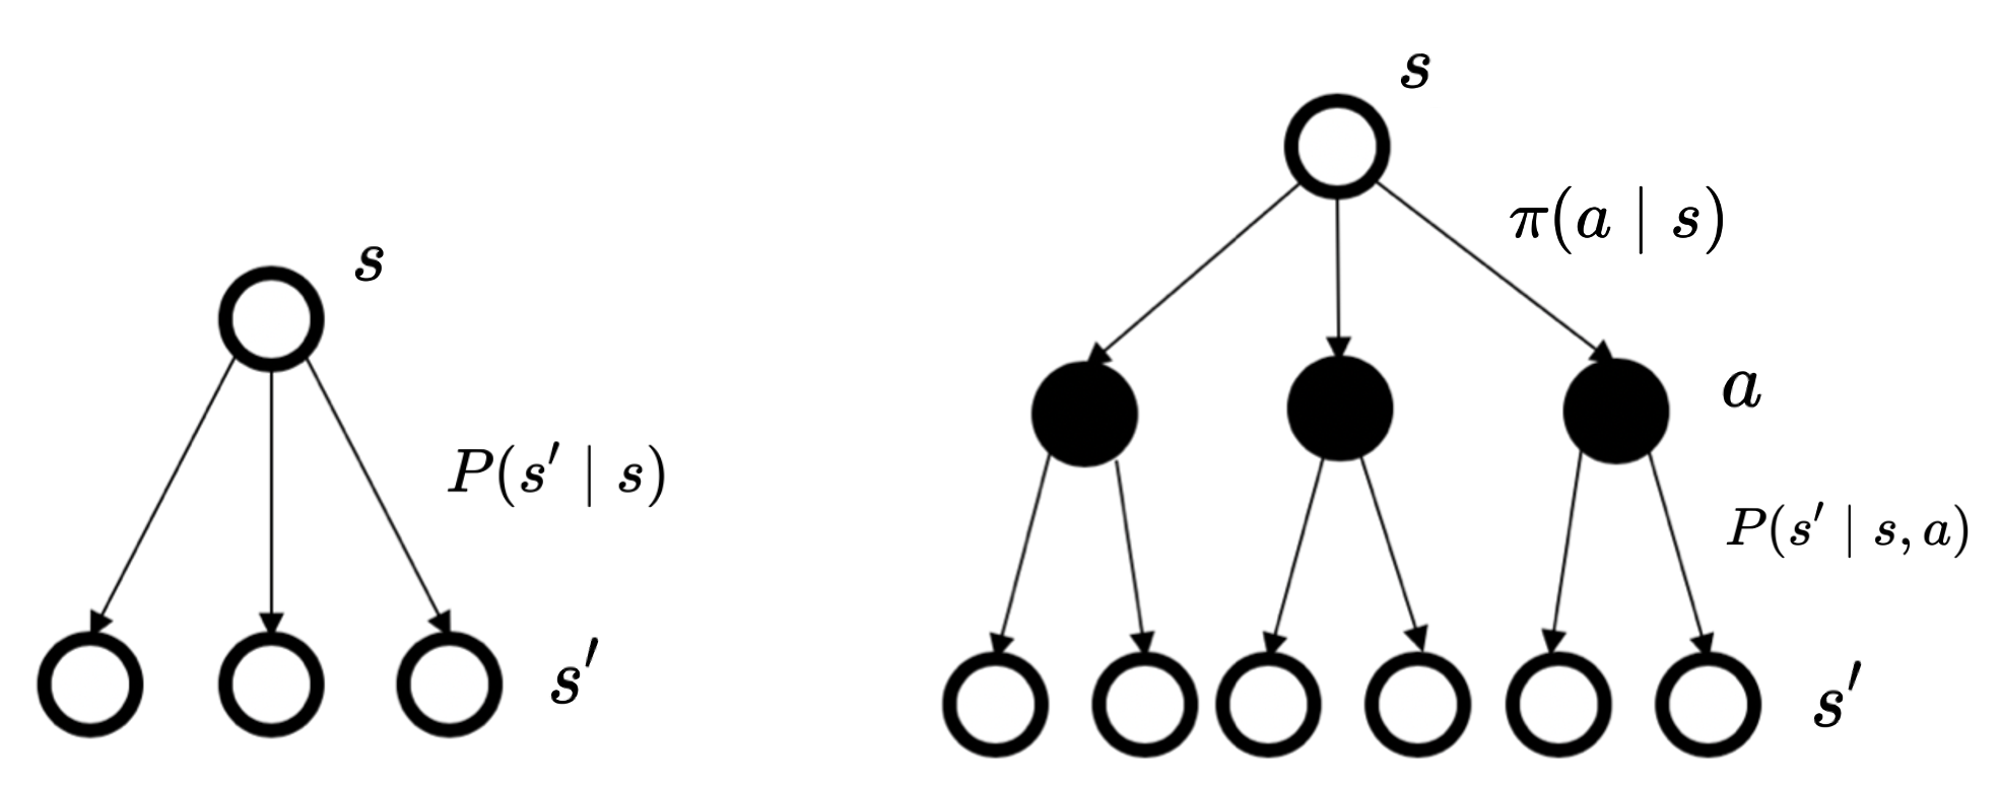
\includegraphics[width=0.6\linewidth]{ch2/figs/2.21.png}
  \caption{马尔可夫决策过程与马尔可夫过程/马尔可夫奖励过程的状态转移的对比}
  \label{fig:fig2.21}
\end{figure}
